\documentclass[10pt]{article}

\usepackage[utf8]{inputenc}
\usepackage[T1]{fontenc}
\usepackage[a4paper,top=0.72in,bottom=0.78in,left=0.82in,right=0.82in]{geometry}
\usepackage{amsmath,amssymb,amsfonts}
\usepackage{array}
\usepackage{booktabs}
\usepackage{caption}
\usepackage{fancyhdr}
\usepackage{float}
\usepackage{hyperref}
\usepackage{listings}
\usepackage[round,authoryear]{natbib}
\usepackage{tabularx}
\usepackage{tikz}
\usepackage{xcolor}
\usetikzlibrary{arrows.meta,positioning,shapes.geometric,fit}

\hypersetup{
  colorlinks=true,
  linkcolor=black,
  citecolor=blue!55!black,
  urlcolor=blue!55!black,
  pdftitle={ReliQuary: Context-Aware Cryptographic Memory and Trust-Gated Multi-Agent Access Control},
  pdfauthor={Swayam Singal and M. Thenmozhi},
  pdfsubject={Context-aware access control and cryptographic memory},
  pdfkeywords={ReliQuary, cryptographic memory, zero trust, post-quantum cryptography, multi-agent systems}
}
\setlength{\parindent}{0pt}
\setlength{\parskip}{0.55em}
\setlength{\tabcolsep}{5pt}
\renewcommand{\arraystretch}{1.15}
\captionsetup{font=small,labelfont=bf}

\pagestyle{fancy}
\fancyhf{}
\lhead{Cureus Journal of Computer Science}
\rhead{ReliQuary}
\cfoot{\thepage}
\setlength{\headheight}{14pt}

\newcommand{\system}{\textsc{ReliQuary}}
\let\cite\citep
\newcommand{\statusimplemented}{\textbf{Implemented}}
\newcommand{\statusoptional}{\textbf{Optional research module}}
\newcommand{\statusproposed}{\textbf{Proposed / not yet validated}}
\newcolumntype{Y}{>{\raggedright\arraybackslash}X}

\lstset{
  basicstyle=\ttfamily\small,
  frame=single,
  breaklines=true,
  columns=fullflexible,
  showstringspaces=false
}

\begin{document}

\begin{center}
{\Large\bfseries ReliQuary: Context-Aware Cryptographic Memory and Trust-Gated Multi-Agent Access Control\par}
\vspace{1.1em}
{\large SWAYAM SINGAL$^{1}$, DR M THENMOZHI$^{2}$\par}
\vspace{0.7em}
{\small
$^{1}$School of Computer Science, VIT Vellore, Vellore, Tamil Nadu, India\\
$^{2}$School of Social Sciences and Languages, VIT Vellore, Vellore, Tamil Nadu, India\\
Corresponding author: Dr M Thenmozhi, \href{mailto:thenmozhi.nisha@vit.ac.in}{thenmozhi.nisha@vit.ac.in}
}
\end{center}

\section*{Abstract}

Modern secret-management systems face two distinct pressures: public-key mechanisms must migrate toward post-quantum standards, while authorization must move beyond static identity and role checks toward continuous evaluation of user, device, location, and behavioral context. This study presents \system, an open-source cryptographic-memory architecture designed to bind disclosure capability to an inspectable authorization process. The architecture combines encrypted vault storage, context-derived trust, multi-agent authorization, threshold key reconstruction, privacy-preserving context hooks, tamper-evident auditing, controlled sharing, and a GPU-rendered decision interface. The implementation uses FastAPI, AES-256-GCM secret envelopes, local-folder/PostgreSQL/S3-compatible adapters, sensitivity-dependent \texttt{allow}, \texttt{redact}, and \texttt{deny} decisions, per-secret passwords, expiring share tokens, Merkle structures, Python consensus modules, Rust/PyO3 cryptographic boundaries, browser and macOS clients, and a Vulkan/Dear ImGui visualizer. Reproducible verification on 13 July 2026 completed 59 Python tests with three service-dependent skips, built the Next.js website, compiled both Rust extension crates, and built the Vulkan visualizer. These results establish software-path viability but do not validate the original AWS-scale latency, machine-learning accuracy, Byzantine fault-injection, or production post-quantum claims. The original evaluation design and numerical claims are therefore retained as marked replication targets rather than current evidence. \system is consequently a functional research platform for context-gated cryptographic memory; production use still requires hardened identity, external key management, real Circom artifacts, standardized PQC migration, independent security review, and replicated large-scale evaluation.

\textbf{Keywords:} cryptographic memory, zero trust, context-aware access control, post-quantum cryptography, zero-knowledge proofs, multi-agent systems, Byzantine fault tolerance, dynamic trust, secret vault, Vulkan

\section*{Introduction}

In modern communication and data-storage systems, the security of public-key cryptography has historically depended on the computational difficulty of integer factorization and discrete logarithms. Shor's algorithm showed that a sufficiently capable quantum computer could solve both classes of problems efficiently, motivating the development and standardization of post-quantum cryptography (PQC) \cite{shor1994,fips204,fips203}. At the same time, network architecture has shifted toward zero-trust models in which no request receives implicit confidence solely because it originates from a familiar network, device, or account \cite{nistzt}. Role-Based Access Control (RBAC) remains useful but is often too rigid to represent rapidly changing context. Attribute-Based Access Control (ABAC) is more expressive, yet large attribute sets create policy-management and conflict-resolution complexity \cite{rbac2000,abac2014,ucon}.

These problems are related. Quantum-resistant encryption protects the mathematical boundary around data, but it cannot determine whether a currently authenticated request should receive the plaintext. Conversely, a sophisticated authorization decision is of limited value if the underlying key-establishment mechanism is vulnerable to future cryptanalytic capability. A future-facing security system must therefore address both cryptographic durability and adaptive disclosure.

This paper proposes \system, a cryptographic-memory system in which access to encrypted state is conditioned on contextual evidence and an auditable decision path. The word \emph{memory} refers to durable encrypted information together with the context, policy, provenance, and access history required to disclose it safely. The system is designed to store ordinary text, files, or folders; evaluate a request against sensitivity and trust requirements; reveal, redact, or deny the requested information; and show the resulting path through browser, macOS, and Vulkan-based interfaces.

The original research concept joined four areas: NIST-directed PQC migration, online zero-knowledge context attestation, heterogeneous multi-agent consensus, and threshold key reconstruction. The present implementation adds a concrete local-first vault, storage adapters, controlled share links, event streaming, and visual inspection. The principal contributions are therefore:

\begin{itemize}
\item A unified architecture that treats cryptography, contextual authorization, auditability, and disclosure as one lifecycle rather than independent services.
\item A privacy-oriented context-attestation design in which device posture, geofencing, and behavioral evidence can be verified without exposing all underlying attributes.
\item A heterogeneous multi-agent decision model with neutral, permissive, strict, and watchdog policy personas, together with a BFT-oriented consensus and threshold-reconstruction design.
\item A deterministic, currently runnable access engine that maps sensitivity and request context to \texttt{allow}, \texttt{redact}, or \texttt{deny}, producing a machine-readable audit event for every decision.
\item A local-first implementation with file/folder secrets, PostgreSQL and S3-compatible adapters, expiring share tokens, and three user interfaces, including a Vulkan/Dear ImGui decision graph.
\item A reproducible verification record that separates current evidence from the unreplicated enterprise-scale performance claims of the earlier manuscript.
\end{itemize}

The remainder of the paper follows the topical organization used by the companion Memory Retrieval Cue manuscript: background and literature are separated from the technical report, methodology, implementation, results, discussion, conclusion, and disclosures.

\section*{Background}

Secret stores traditionally enforce access through possession of a password, token, device key, or role. Those controls answer whether a principal has presented a recognized credential; they do not necessarily answer whether the present request is reasonable. A credential may be stolen, a device may be compromised, or a legitimate account may request an unusual resource from an implausible location. Zero-trust architecture responds by evaluating subjects, assets, and resources at each access boundary rather than treating network location as a sufficient trust signal \cite{nistzt,nistztimpl}.

Post-quantum migration introduces a second design concern. NIST standardized ML-KEM in FIPS 203 and ML-DSA in FIPS 204 in August 2024 \cite{fips204,fips203}. The repository currently contains a Kyber KEM implementation and a Falcon signature implementation through Rust crates. Kyber is the predecessor family of standardized ML-KEM. Falcon was selected for future standardization as FN-DSA/FIPS 206, but it is not yet a finalized FIPS standard \cite{nistpqc}. The implementation must therefore be described as PQC-capable research code, not as a fully NIST-compliant production boundary.

Zero-knowledge proofs (ZKPs) provide a way to prove a statement without exposing the witness used to establish it. In access control, this can permit a client to prove that a device or location satisfies policy without submitting every raw attribute. Practical use is complicated by circuit design, trusted setup requirements for some proving systems, proving latency, artifact management, and the need to bind proofs to fresh requests \cite{zerocash2014,zkpsurvey}.

Multi-agent systems provide another means of avoiding a monolithic policy decision. Agents can represent distinct risk attitudes and inspect the same evidence from different perspectives. However, ordinary majority voting is insufficient when agents may fail, equivocate, or become compromised. Practical Byzantine Fault Tolerance (PBFT) provides a formal basis for reaching agreement when a bounded number of participants behave arbitrarily \cite{pbft,lamport1982}.

\section*{Literature Review}

\subsection*{Post-Quantum Cryptography Integration}

The NIST PQC standardization process established lattice-based cryptography as a practical foundation for quantum-resistant key establishment and signatures \cite{lwerings,nistir8413,fips204,fips203}. Existing research has examined standalone performance and integration into transport protocols such as TLS \cite{pqtls}. Most integration work remains protocol-level: a quantum-resistant primitive replaces a classical primitive while the surrounding authorization model remains unchanged.

\textbf{Research gap:} Cryptographic migration alone does not address contextual misuse of a valid identity. There remains a need for systems in which post-quantum key capability participates in the authorization lifecycle rather than operating as an isolated replacement.

\textbf{ReliQuary contribution:} The target architecture distributes key capability to an authorization quorum and authenticates inter-agent decisions. The current Rust boundary provides Kyber and Falcon operations, while the paper explicitly recognizes the need to migrate to final standardized parameter sets and independently validated libraries.

\subsection*{Zero-Knowledge Proofs in Access Management}

ZKPs have been applied to privacy-preserving payments, decentralized identity, and credential validation \cite{zerocash2014,didcore}. These deployments often concern stable or comparatively long-lived attributes.

\textbf{Research gap:} Ephemeral, high-rate attributes such as current device health, geolocation bounds, and behavioral anomalies are difficult to verify synchronously. Offline or asynchronous proofs do not naturally fit a low-latency authorization loop \cite{zkpsurvey}.

\textbf{ReliQuary contribution:} The proposed protocol creates request-bound proofs for contextual predicates and makes proof validity an input to watchdog-agent policy. The repository includes a deterministic development proof path and external Circom/SnarkJS hooks; real proving and verification artifacts remain deployment requirements.

\subsection*{Adaptive Trust Management}

Limitations of static RBAC and ABAC have motivated dynamic trust engines that aggregate heterogeneous signals into continuous risk estimates \cite{rbac2000,abac2014,ucon,mltrust}. A common approach uses machine learning to model nonlinear interaction among device, location, time, and behavior.

\textbf{Research gap:} Centralized trust engines create a single decision point and can conceal conflicts among signals. Models also drift, inherit bias from their labels, and can be manipulated by gradual behavioral poisoning.

\textbf{ReliQuary contribution:} The implemented trust scorer exposes weighted factors and explanations, while the proposed extension uses a calibrated classifier. Final disclosure remains subject to a separate sensitivity-aware policy and can be mediated by multiple agents.

\subsection*{Multi-Agent Systems for Security Enforcement}

Multi-agent systems have been studied for intrusion detection, threat hunting, and distributed monitoring because they support parallelism and autonomy \cite{masintro}. These applications are commonly asynchronous and reactive.

\textbf{Research gap:} Embedding heterogeneous agents in a synchronous, latency-sensitive authorization path requires bounded-time behavior, signed messages, consistent policy interpretation, and failure handling.

\textbf{ReliQuary contribution:} The research design formalizes authorization as a BFT-oriented state machine. Agents emit structured decisions and confidence values, while a quorum outcome gates disclosure and, in the target architecture, key reconstruction.

\section*{Technical Report: System Architecture}

\system is organized as five conceptual layers. This separation supports local operation today and a distributed deployment path without pretending that every target component is already production-hardened.

\begin{enumerate}
\item \textbf{Client layer:} browser, macOS desktop, Vulkan/Dear ImGui console, and language SDKs. Clients collect user intent and context, but do not authoritatively decide disclosure.
\item \textbf{API and identity layer:} the FastAPI entrypoint exposes health, authentication, context, trust, access, memory, sharing, agent, audit, and vault routes.
\item \textbf{Decision layer:} sensitivity thresholds, trust evaluation, multi-agent orchestration, and event generation determine whether a result is fully revealed, metadata-only, existence-only, or hidden.
\item \textbf{Cryptographic layer:} AES-256-GCM protects payload envelopes; Rust/PyO3 modules expose Kyber, Falcon, and Merkle operations; Circom/SnarkJS remains an external proving path.
\item \textbf{Storage layer:} local directories, PostgreSQL, or S3-compatible object storage persist vault and secret records. Audit events are written to JSONL and Merkle-oriented log structures.
\end{enumerate}

\begin{figure}[ht]
\centering
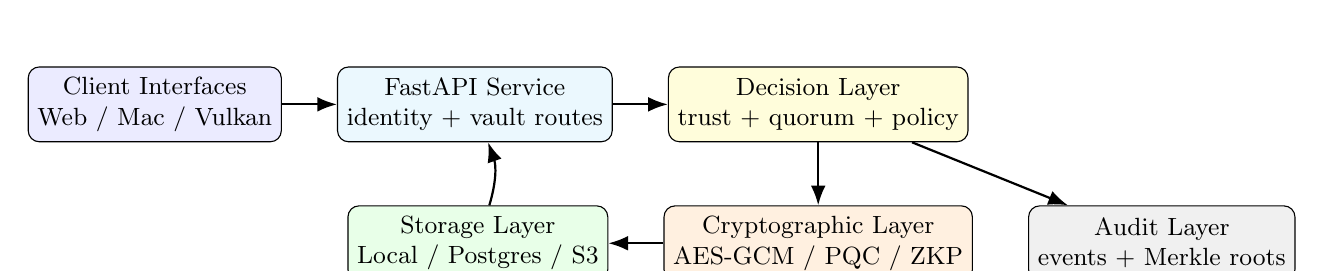
\begin{tikzpicture}[
box/.style={draw,rounded corners,align=center,minimum height=0.95cm,minimum width=2.55cm,font=\small},
arrow/.style={-{Latex[length=2.5mm]},thick}
]
\node[box,fill=blue!8] (clients) {Client Interfaces\\Web / Mac / Vulkan};
\node[box,fill=cyan!8,right=0.7cm of clients] (api) {FastAPI Service\\identity + vault routes};
\node[box,fill=yellow!14,right=0.7cm of api] (decision) {Decision Layer\\trust + quorum + policy};
\node[box,fill=orange!12,below=0.8cm of decision] (crypto) {Cryptographic Layer\\AES-GCM / PQC / ZKP};
\node[box,fill=green!9,left=0.7cm of crypto] (storage) {Storage Layer\\Local / Postgres / S3};
\node[box,fill=gray!12,right=0.7cm of crypto] (audit) {Audit Layer\\events + Merkle roots};
\draw[arrow] (clients) -- (api);
\draw[arrow] (api) -- (decision);
\draw[arrow] (decision) -- (crypto);
\draw[arrow] (crypto) -- (storage);
\draw[arrow] (decision) -- (audit);
\draw[arrow,bend right=18] (storage) to (api);
\end{tikzpicture}
\caption{High-level \system architecture. The API remains the security authority; interfaces display decisions but do not bypass them.}
\label{fig:architecture}
\end{figure}

\subsection*{Enterprise Integration}

The target design can operate as a Policy Enforcement Point downstream of an enterprise identity provider, consistent with NIST zero-trust concepts \cite{nistzt}. LDAP, SAML, OAuth 2.0, WebAuthn, or decentralized-identifier assertions can establish identity, after which \system evaluates request context and resource policy. A client SDK or sidecar can mediate application access. This enterprise arrangement is an architectural target; the current local setup uses development-oriented authentication paths and must not be deployed on an untrusted network without configuration changes.

\subsection*{Threat Model}

The design considers the following adversaries:

\begin{itemize}
\item \textbf{Passive quantum adversary:} records ciphertext today for future decryption. The target mitigation is standardized post-quantum key establishment and signatures.
\item \textbf{Active network adversary:} reads, modifies, replays, or drops messages. Mitigations include authenticated transport, fresh request binding, signed messages, and replay-resistant proof statements.
\item \textbf{Malicious or compromised client:} presents valid identity credentials while attempting access beyond legitimate need. Mitigations include contextual trust, sensitivity thresholds, per-secret passwords, and fail-closed decisions.
\item \textbf{Compromised agent:} submits arbitrary or conflicting decisions. A BFT quorum of size $n \geq 3f+1$ is intended to tolerate up to $f$ Byzantine participants \cite{pbft}.
\item \textbf{Insider or storage adversary:} reads backing storage or tampers with audit records. Payload encryption limits plaintext exposure; Merkle-rooted logging supports tamper evidence \cite{merkle1989}.
\item \textbf{Share-link attacker:} obtains or guesses a token. Expiry, view limits, optional share passwords, and per-secret access passwords reduce but do not eliminate risk.
\end{itemize}

Physical side channels, coercion, compromised operating-system kernels, malicious dependency updates, and denial of service are outside the protection demonstrated by the current repository. High-assurance deployments require an HSM or Secure Enclave strategy, dependency review, key rotation, backups, rate limits, and operational monitoring.

\section*{Methodology}

\subsection*{Context and Trust Representation}

The implemented trust scorer calculates five interpretable factors: context verification $c$, historical behavior $h$, inverse risk $r$, consistency $s$, and recency $t$. With the default configuration, the normalized score is

\begin{equation}
T = 0.30c + 0.25h + 0.20r + 0.15s + 0.10t,
\qquad T \in [0,1].
\end{equation}

The API-facing access engine represents the score on $[0,100]$ and applies explicit penalties for non-owner requests, remote access without a trusted local session, missing device verification, and missing biometric or explicit high-trust confirmation. This deterministic path is the current decision authority and is easier to audit than an opaque classifier.

The original adaptive model is retained as a research extension. It derives a feature vector $\mathbf{f}=[f_1,f_2,f_3,f_4]$ from device consistency, temporal anomaly, geographic velocity, and behavioral anomaly. A calibrated classifier $M$ estimates

\begin{equation}
T_{ML}=100\,P_M(\text{trustworthy}\mid\mathbf{f}).
\end{equation}

The earlier manuscript proposed a random forest and Isolation Forest trained on a rolling 30-day window. That process remains valid as an evaluation design, but the repository does not contain the claimed enterprise dataset or an accepted trained model. Any future model must use subject- or organization-held-out validation, calibration, drift monitoring, and analyst-reviewed labels.

\subsection*{Sensitivity-Aware Disclosure}

Each resource receives one of five sensitivity levels. Table~\ref{tab:thresholds} shows the current policy thresholds.

\begin{table}[ht]
\centering
\caption{Implemented sensitivity thresholds and disclosure behavior}
\label{tab:thresholds}
\begin{tabularx}{\textwidth}{l c Y}
\toprule
\textbf{Sensitivity} & \textbf{Required score} & \textbf{Policy intent}\\
\midrule
Public & 0 & Low-risk data may be disclosed, subject to request validation.\\
Private & 50 & Owner-oriented data requires moderate contextual trust.\\
Sensitive & 75 & High trust and a verified device are expected.\\
Secret & 90 & Verified device and biometric or explicit confirmation are expected.\\
Sealed & 101 & Direct value disclosure is impossible under the current policy.\\
\bottomrule
\end{tabularx}
\end{table}

The engine returns one of three decisions: \texttt{allow} reveals the requested value; \texttt{redact} reveals only metadata or existence; and \texttt{deny} reveals no useful resource information. The exact reason list is persisted with the event.

\begin{figure}[ht]
\centering
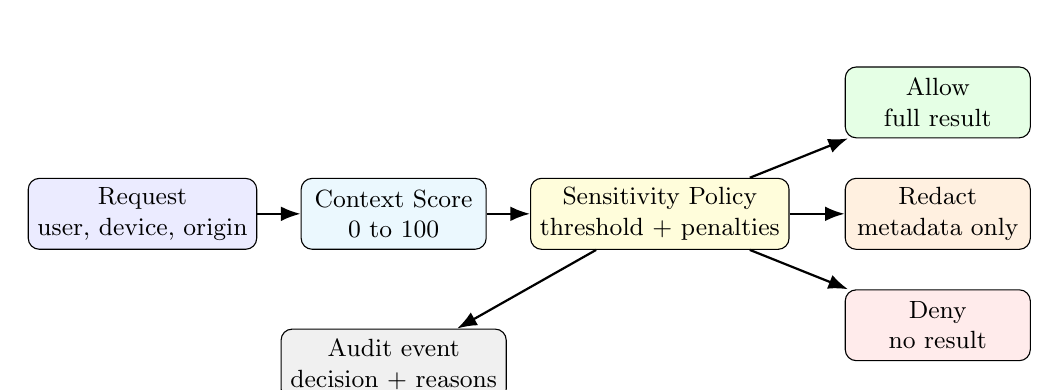
\begin{tikzpicture}[
box/.style={draw,rounded corners,align=center,minimum height=0.9cm,minimum width=2.35cm,font=\small},
arrow/.style={-{Latex[length=2.5mm]},thick}
]
\node[box,fill=blue!8] (request) {Request\\user, device, origin};
\node[box,fill=cyan!8,right=0.55cm of request] (score) {Context Score\\$0$ to $100$};
\node[box,fill=yellow!14,right=0.55cm of score] (policy) {Sensitivity Policy\\threshold + penalties};
\node[box,fill=green!10,above right=0.5cm and 0.7cm of policy] (allow) {Allow\\full result};
\node[box,fill=orange!12,right=0.7cm of policy] (redact) {Redact\\metadata only};
\node[box,fill=red!8,below right=0.5cm and 0.7cm of policy] (deny) {Deny\\no result};
\node[box,fill=gray!12,below=1.0cm of score] (event) {Audit event\\decision + reasons};
\draw[arrow] (request) -- (score);
\draw[arrow] (score) -- (policy);
\draw[arrow] (policy) -- (allow);
\draw[arrow] (policy) -- (redact);
\draw[arrow] (policy) -- (deny);
\draw[arrow] (policy) -- (event);
\end{tikzpicture}
\caption{Implemented access-decision path used by the API and all three interfaces.}
\label{fig:decision}
\end{figure}

\subsection*{Heterogeneous Multi-Agent Consensus}

The research design uses seven agents and targets tolerance of two Byzantine faults because $7\geq 3(2)+1$. Four policy personas provide deliberately different risk attitudes:

\begin{table}[ht]
\centering
\caption{Agent persona policy definitions retained from the original design}
\label{tab:personas}
\begin{tabularx}{\textwidth}{l c Y}
\toprule
\textbf{Persona} & \textbf{Target count} & \textbf{Decision rule}\\
\midrule
Neutral & 2 & Grant if $T\geq50$; otherwise deny.\\
Permissive & 1 & Grant if $T\geq30$; flag $30\leq T<50$ for audit.\\
Strict & 2 & Grant if $T\geq70$; otherwise deny.\\
Watchdog & 2 & Grant only if $T\geq60$ and the context proof is valid; alert on proof failure.\\
\bottomrule
\end{tabularx}
\end{table}

The implemented test configuration also exercises smaller four-agent networks. The generic constraint $n\geq3f+1$ is calculated by the consensus module. The conceptual protocol is:

\begin{minipage}{\textwidth}
\begin{lstlisting}[caption={BFT-oriented multi-agent authorization protocol},label={alg:consensus}]
INPUT: request r, trust T, proof pi, agents A, quorum q = 2f + 1
1. Orchestrator broadcasts (r, T, pi) to each agent.
2. Every agent applies its persona policy and returns
   (decision, confidence, authenticated response).
3. Invalid or late responses are excluded.
4. If fewer than q valid responses remain, return DENY.
5. Compare confidence-weighted grant and deny evidence.
6. Return the fail-closed consensus decision and audit record.
\end{lstlisting}
\end{minipage}

\begin{figure}[ht]
\centering
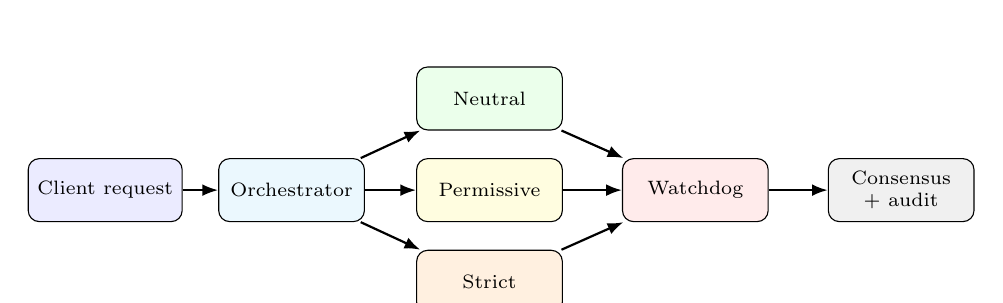
\begin{tikzpicture}[
box/.style={draw,rounded corners,align=center,minimum height=0.8cm,minimum width=1.85cm,font=\scriptsize},
arrow/.style={-{Latex[length=2mm]},thick}
]
\node[box,fill=blue!8] (client) {Client request};
\node[box,fill=cyan!8,right=0.45cm of client] (orch) {Orchestrator};
\node[box,fill=green!8,above right=0.35cm and 0.65cm of orch] (neutral) {Neutral};
\node[box,fill=yellow!12,right=0.65cm of orch] (perm) {Permissive};
\node[box,fill=orange!12,below right=0.35cm and 0.65cm of orch] (strict) {Strict};
\node[box,fill=red!8,right=0.75cm of perm] (watch) {Watchdog};
\node[box,fill=gray!12,right=0.75cm of watch] (result) {Consensus\\+ audit};
\draw[arrow] (client) -- (orch);
\draw[arrow] (orch) -- (neutral);
\draw[arrow] (orch) -- (perm);
\draw[arrow] (orch) -- (strict);
\draw[arrow] (neutral) -- (watch);
\draw[arrow] (perm) -- (watch);
\draw[arrow] (strict) -- (watch);
\draw[arrow] (watch) -- (result);
\end{tikzpicture}
\caption{Heterogeneous agent evaluation and consensus sequence. In production, each response must be authenticated and bound to the request.}
\label{fig:quorum}
\end{figure}

\subsection*{Consensus-Gated Threshold Cryptography}

The target key-management design combines Shamir's Secret Sharing (SSS) with the agent quorum \cite{shamir1979}. A vault key $K$ is split into $n$ shares with threshold $t=2f+1$. Share $s_i$ is encapsulated for agent $a_i$. Reconstruction proceeds only after an approving quorum:

\begin{lstlisting}[caption={Consensus-gated key reconstruction},label={alg:keyrec}]
INPUT: consensus D, approving agents A+, threshold t
1. If D is not GRANT or |A+| < t, return failure.
2. Request one protected key share from each approving agent.
3. Authenticate each response and decapsulate its share.
4. Reconstruct K from any valid threshold subset.
5. Use K only for the authorized operation, then erase transient copies.
\end{lstlisting}

The repository tests SSS reconstruction and rejection with insufficient shares. Full coupling between distributed PQC-protected shares and every vault read remains a target architecture rather than a completed production key-management system.

\subsection*{Zero-Knowledge Context Attestation}

The intended online protocol binds a proof to a request nonce, policy identifier, and short validity interval. Public inputs contain only the predicates needed by policy; private inputs contain raw contextual evidence. A verifier supplies the result to the trust engine and watchdog agents. The current repository supports deterministic development envelopes and optional Circom/SnarkJS integration. Mock batch verifiers are not cryptographic evidence and are excluded from production claims.

\subsection*{Secret Storage and Sharing}

Vault records can contain text, a single file, or a folder. File and folder inputs are packaged for transport and encrypted into a secret envelope. A secret may additionally require its own password. Share tokens contain an expiry, maximum view count, and optional share password; opening a token may also require the underlying secret password. Cross-device sharing works only when both devices can reach the same API and backing storage. The repository is not a decentralized global relay or a replacement for end-to-end messaging protocols.

\begin{figure}[ht]
\centering
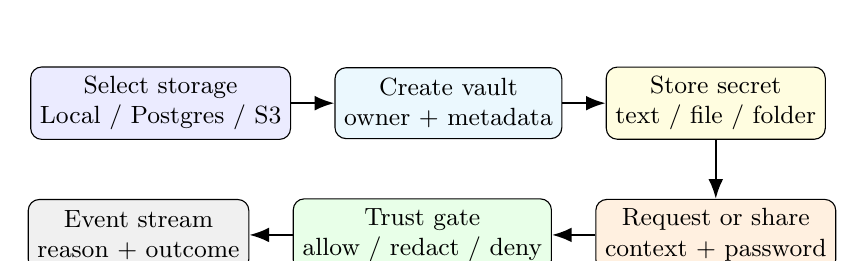
\begin{tikzpicture}[
box/.style={draw,rounded corners,align=center,minimum height=0.9cm,minimum width=2.2cm,font=\small},
arrow/.style={-{Latex[length=2.5mm]},thick}
]
\node[box,fill=blue!8] (storage) {Select storage\\Local / Postgres / S3};
\node[box,fill=cyan!8,right=0.55cm of storage] (vault) {Create vault\\owner + metadata};
\node[box,fill=yellow!12,right=0.55cm of vault] (secret) {Store secret\\text / file / folder};
\node[box,fill=orange!12,below=0.75cm of secret] (request) {Request or share\\context + password};
\node[box,fill=green!9,left=0.55cm of request] (gate) {Trust gate\\allow / redact / deny};
\node[box,fill=gray!12,left=0.55cm of gate] (audit) {Event stream\\reason + outcome};
\draw[arrow] (storage) -- (vault);
\draw[arrow] (vault) -- (secret);
\draw[arrow] (secret) -- (request);
\draw[arrow] (request) -- (gate);
\draw[arrow] (gate) -- (audit);
\end{tikzpicture}
\caption{End-to-end vault workflow represented in the GUI and API.}
\label{fig:vaultflow}
\end{figure}

\section*{Implementation}

\subsection*{Backend and Storage}

The canonical backend entrypoint is \texttt{apps.api.main:app}. It exposes routers for authentication, context, trust, access decisions, local-memory indexing, sharing, agents, audit, and vault operations. The local adapter provides a clone-and-run path; PostgreSQL demonstrates a real queryable database; S3-compatible storage supports object-store deployments when credentials and bucket policy are configured. IPFS and Arweave boundaries fail explicitly until configured instead of silently pretending to persist data.

Secret values use AES-GCM envelopes. GCM supplies authenticated encryption, so tampering with either ciphertext or authentication tag is detected \cite{aesgcm}. The production weakness is not the basic primitive but key lifecycle: development-oriented local key configuration must be replaced with an OS keychain, Secure Enclave/HSM, or managed KMS design before real high-value secrets are stored.

\subsection*{Rust Cryptographic Boundary}

Two PyO3 crates are present. \texttt{reliquary\_encryptor} exposes AES-GCM, Kyber, Falcon, hashing, and zeroization-related operations; \texttt{reliquary\_merkle} exposes Merkle functionality. The Python wrapper fails loudly when optional PQC modules are unavailable rather than substituting fake post-quantum output. Both crates compile successfully in the current verification, but each presently reports zero native Rust unit tests. Python integration tests cover available round trips and tamper rejection; audited test vectors and native crate tests remain necessary.

\subsection*{Web, macOS, and Vulkan Interfaces}

The browser console and native Tk-based macOS GUI provide storage initialization, vault creation, secret operations, trust controls, and event inspection. They are clients of the same API and do not store authoritative secret state themselves.

The Vulkan application is implemented in \texttt{visualizer/vulkan/src/main.cpp}. GLFW creates the window and surface; Vulkan initializes the instance, device, swapchain, image views, render pass, framebuffers, command buffers, and synchronization; Dear ImGui supplies the controls. On macOS the path uses MoltenVK. The graph displays storage, trust-gate, request, and result nodes while API calls create vaults, store text/files/folders, request secrets, create share tokens, simulate remote attackers, and refresh events. Vulkan is therefore the native visual-computing and interaction layer, not the cryptographic or policy engine \cite{vulkan,imgui}.

\begin{figure}[ht]
\centering
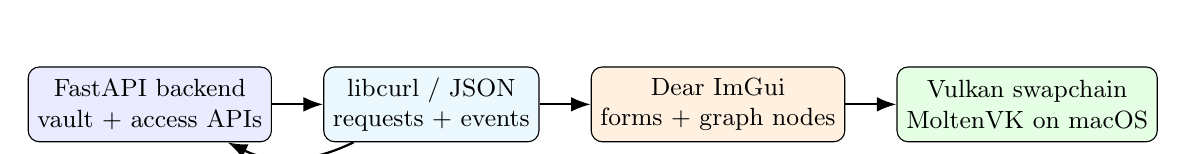
\begin{tikzpicture}[
box/.style={draw,rounded corners,align=center,minimum height=0.95cm,minimum width=2.55cm,font=\small},
arrow/.style={-{Latex[length=2.5mm]},thick}
]
\node[box,fill=blue!8] (api) {FastAPI backend\\vault + access APIs};
\node[box,fill=cyan!8,right=0.65cm of api] (http) {libcurl / JSON\\requests + events};
\node[box,fill=orange!12,right=0.65cm of http] (imgui) {Dear ImGui\\forms + graph nodes};
\node[box,fill=green!10,right=0.65cm of imgui] (vk) {Vulkan swapchain\\MoltenVK on macOS};
\draw[arrow] (api) -- (http);
\draw[arrow] (http) -- (imgui);
\draw[arrow] (imgui) -- (vk);
\draw[arrow,bend left=26] (http) to (api);
\end{tikzpicture}
\caption{Role of Vulkan in \system: GPU rendering of an API-backed trust graph and unified control console.}
\label{fig:vulkan}
\end{figure}

\subsection*{Implementation Boundaries}

\begin{table}[ht]
\centering
\caption{Current implementation status}
\label{tab:status}
\begin{tabularx}{\textwidth}{l l Y}
\toprule
\textbf{Area} & \textbf{Status} & \textbf{Evidence and boundary}\\
\midrule
Vault API and storage & \statusimplemented & Local, PostgreSQL, and S3-compatible adapters; text/file/folder payload flows.\\
Access decisions & \statusimplemented & Deterministic sensitivity thresholds, penalties, allow/redact/deny, reasoned events.\\
Sharing & \statusimplemented & Expiring, view-limited tokens with optional share and secret passwords.\\
Audit structures & \statusimplemented & JSONL decision events and Merkle-oriented log/proof modules.\\
Multi-agent consensus & \statusoptional & Runnable Python modules and tests; not a hardened distributed seven-node deployment.\\
PQC & \statusoptional & Rust Kyber/Falcon paths; standards migration and independent validation required.\\
ZKP & \statusoptional & Development proof envelopes and external Circom hooks; mock verifier paths remain.\\
Vulkan visualizer & \statusimplemented & Native swapchain and ImGui API console build successfully on macOS.\\
Enterprise IAM/Kubernetes & \statusproposed & Architectural integration target, not current deployment evidence.\\
\bottomrule
\end{tabularx}
\end{table}

\section*{Evaluation and Results}

\subsection*{Reproducible Repository Verification}

The current evaluation asks a narrower and more defensible question than the original manuscript: do the implemented research paths build and behave consistently from the repository? Table~\ref{tab:verification} records the verification performed on 13 July 2026 on macOS.

\begin{table}[ht]
\centering
\caption{Current reproducible verification results}
\label{tab:verification}
\begin{tabularx}{\textwidth}{l c Y}
\toprule
\textbf{Verification surface} & \textbf{Outcome} & \textbf{Interpretation}\\
\midrule
Python test matrix & 59 passed, 3 skipped & Covers API routes, trust and access outcomes, vault persistence, sharing, AES-GCM, Merkle behavior, consensus, and threshold reconstruction. Three external-service-dependent SSS tests were skipped.\\
Python warnings & 30 & Six timezone deprecations and 24 LangGraph API deprecations; non-fatal but should be removed.\\
Website production build & Passed & Next.js compiled, type-checked, and generated the root and not-found static routes.\\
Rust encryptor crate & Built; 0 native tests & Compilation succeeds; absence of Rust unit tests limits native-boundary assurance.\\
Rust Merkle crate & Built; 0 native tests & Compilation succeeds; native test vectors are still required.\\
Vulkan visualizer & Passed & CMake configured and built Dear ImGui and the \texttt{reliquary\_vulkan\_visualizer} target.\\
\bottomrule
\end{tabularx}
\end{table}

The tests demonstrate important behavior rather than only importability. High-trust owner requests for secret resources are allowed; low-trust remote requests are denied; near-threshold requests can be redacted; access events are exposed to visualizers; tampered AES-GCM ciphertext and tags fail; local storage survives manager recreation; file secrets can be shared through bounded tokens; and insufficient threshold shares cannot reconstruct a secret.

These results establish a functional software research platform. They do not establish resistance to side channels, security of every dependency, correctness of unexecuted mock paths, high availability, formal BFT safety, or production-scale performance.

\subsection*{Security Review Findings}

The repository's internal security report reaches a deliberately severe conclusion: the project is promising but not yet production-trustworthy. The strongest evidence is runnable verification and the existence of real storage and cryptographic boundaries. The principal weaknesses are prototype markers, development defaults, mock ZK paths, local key management, wildcard CORS, incomplete native tests, and uneven depth across the broad API surface. The earlier score graphic is intentionally excluded from this paper because a single composite number suggests a precision that the audit methodology does not support.

\subsection*{Original Enterprise Evaluation Design}

The original manuscript proposed a standardized AWS study. Three \texttt{m6i.xlarge} nodes would host the control plane. Seven dedicated \texttt{m6i.2xlarge} instances would host the consensus agents, while five \texttt{c6i.4xlarge} load generators would use k6. Each test would run for 15 minutes after a five-minute warm-up, with geometric concurrency ramps, three independent runs, and 95\% confidence intervals.

The retained legacy stack specified Kubernetes 1.28 on Bottlerocket OS, Python 3.10 with \texttt{asyncio} and \texttt{uvloop}, Open Quantum Safe \texttt{liboqs} 0.8.0, and an original PBFT implementation. It also named FoundationDB 7.3.23 as the primary datastore, although the architecture section named PostgreSQL, Redis, and S3-compatible storage. That inconsistency is corrected in the current implementation by documenting local-folder, PostgreSQL, and S3-compatible adapters as the supported storage paths; Redis and FoundationDB remain deployment ideas rather than evaluated dependencies.

The proposed baseline substitutes RSA-2048, ECDSA P-256, and a centralized decision engine for the PQC, ZKP, and BFT paths. The original trust study specified three datasets: 10,000 synthetic login samples with injected attacks, 5,000 de-identified enterprise VPN traces with analyst labels, and 2,000 adversarial patterns. This remains a useful evaluation protocol, but the datasets, infrastructure logs, raw measurements, and analysis code required to reproduce the reported values are absent from the repository.

\subsection*{Legacy Claims Requiring Replication}

To preserve the original paper without presenting unsupported numbers as fact, Table~\ref{tab:legacyclaims} records its major empirical claims and their current evidence status. The detailed historical tables are retained in the appendix.

\begin{table}[ht]
\centering
\caption{Validation status of numerical claims from the original manuscript}
\label{tab:legacyclaims}
\begin{tabularx}{\textwidth}{Y l Y}
\toprule
\textbf{Original claim} & \textbf{Current status} & \textbf{Evidence needed}\\
\midrule
45.2 ms mean authorization latency at 1,000 clients & Unreplicated & Raw k6 output, infrastructure definition, versions, run logs, and statistical analysis.\\
97.0\% F1 on real enterprise traces & Unreplicated & Licensed dataset, labels, split protocol, trained model, calibration, and held-out predictions.\\
Correct operation with two Byzantine agents & Partially exercised & Distributed seven-node fault injection with equivocation, delay, crash, and partition traces.\\
5.2 ms ZKP generation and 1.8 ms verification & Unreplicated & Circuit, proving system, artifact hashes, hardware, and benchmark harness.\\
Enterprise deployment readiness & Not supported & Threat modeling, penetration test, key management, secure defaults, CI evidence, incident procedures, and external review.\\
\bottomrule
\end{tabularx}
\end{table}

\section*{Discussion}

\subsection*{What the Project Achieves}

\system now demonstrates more than a website or isolated cryptographic example. A user can initialize a real local or PostgreSQL-backed store, create a vault, store text or packaged file/folder secrets, add a secret-specific password, evaluate access under explicit context, observe an allow/redact/deny result, inspect the audit event, and create a bounded share token. The same flow is available through the API, browser interface, native macOS GUI, and Vulkan visualizer.

The visual layer is particularly valuable for research communication. Security failures are often invisible because an application returns only an HTTP status. The graph instead exposes the relationship among storage, resource sensitivity, trust evidence, decision, and visible result. A remote attacker simulation can be compared with a verified local request without changing the backend policy engine.

\subsection*{Scientific and Security Validity}

The strongest scientific framing is that \system is a testable architecture for context-gated cryptographic memory. It is not yet evidence that a multi-agent quorum is superior to a carefully engineered deterministic policy engine, nor that machine learning improves authorization safety. Those hypotheses require controlled baselines, ablation studies, calibrated error analysis, and adversarial testing.

Trust scores must not be interpreted as objective truth about a person. They are policy inputs derived from measurements and assumptions. False acceptance can expose a secret; false rejection can make critical data unavailable. Every future learned model therefore requires calibration, subgroup analysis where lawful and appropriate, drift monitoring, and a deterministic fail-closed fallback.

Likewise, the presence of Kyber, Falcon, ZKP, and Merkle modules does not automatically make the whole application post-quantum, zero-knowledge, or tamper-proof. Security properties apply only when algorithms, parameters, keys, proof artifacts, bindings, storage, transport, and operational procedures are all correct.

\subsection*{Limitations}

The current study has the following limitations:

\begin{itemize}
\item The original enterprise benchmark and trust datasets are unavailable, so historical latency and accuracy values are unverified.
\item Rust crates compile but contain no native unit-test suites; cryptographic assurance relies partly on Python integration tests.
\item The ZK subsystem contains deterministic and mock paths. A production claim requires real circuits, ceremony/artifact documentation where applicable, and tamper/replay tests.
\item The Python consensus implementation is not equivalent to a geographically distributed, adversarially tested PBFT deployment.
\item Local key management and permissive development configuration are inappropriate for production secrets.
\item Share links depend on a reachable central API and are not an end-to-end encrypted peer-to-peer messaging system.
\item The current evaluation demonstrates software behavior, not formal security proof or certification.
\end{itemize}

\subsection*{Future Work}

The immediate research agenda is ordered by evidentiary value. First, remove mock verification from production routes, add Rust test vectors, migrate PQC interfaces to finalized standardized constructions, and place keys behind macOS Keychain/Secure Enclave or an HSM/KMS abstraction. Second, deploy the seven-agent topology and publish a fault-injection harness covering crash, equivocation, delay, replay, and network partition. Third, release a lawful, de-identified trust dataset or a complete synthetic generator, use organization-held-out evaluation, calibrate probabilities, and report false acceptance and false rejection with confidence intervals. Fourth, run the preserved AWS or equivalent Apple-container-compatible benchmark protocol and publish all raw outputs. Fifth, commission external code review and penetration testing before any enterprise-readiness claim.

Longer-term work can evaluate reinforcement learning for adaptive agent thresholds and external anchoring of Merkle roots. Both ideas require caution: adaptive policies can become unstable or exploitable, while public anchoring proves only that a root existed, not that the logged event was true.

\section*{Conclusions}

This paper presented \system as a context-aware cryptographic-memory architecture that couples encrypted storage to explicit disclosure policy, interpretable trust evidence, multi-agent authorization research, threshold reconstruction, and auditable visualization. The work preserves the original post-quantum, zero-knowledge, and BFT research direction while aligning every present-tense claim with the repository.

The verified result is a functional local-first research platform: 59 Python tests pass, the web console builds, the Rust extension crates compile, and the Vulkan/Dear ImGui application builds. Users can create vaults, store text/files/folders, apply per-secret passwords, request or share secrets, and observe why disclosure was allowed, redacted, or denied. The unverified result is the earlier claim of enterprise-scale latency, 97\% trust-classification F1, complete two-fault Byzantine resilience, and production readiness. Those claims are retained as explicit replication targets.

The central contribution is therefore architectural and experimental: \system supplies a concrete environment in which cryptographic durability, contextual authorization, heterogeneous decision-making, storage, sharing, and visual explanation can be tested together. Its path to production is measurable, but not yet complete.

\section*{Additional Information}

\subsection*{Disclosures}

\textbf{Human subjects:} The repository verification and software study reported here did not involve human participants or tissue. Any future use of enterprise behavioral traces or biometric context must receive appropriate institutional, legal, and privacy review.

\textbf{Animal subjects:} This study did not involve animal subjects or tissue.

\textbf{Conflicts of interest:} The authors declare no financial relationship or other activity that appears to have influenced the submitted work.

\textbf{Funding:} No external financial support is claimed for the repository verification reported in this paper.

\textbf{Data and code availability:} The implementation, tests, build scripts, and documentation are maintained in the open-source ReliQuary repository. Historical enterprise datasets and AWS benchmark artifacts described by the original manuscript are not currently available and are therefore not treated as reproducible evidence.

\section*{Appendix: Historical Evaluation Record}
This appendix preserves the original manuscript's numerical tables for traceability. Values in this appendix are \textbf{legacy, unreplicated claims}; they must not be cited as results of the current repository verification.

\begin{table}[H]
\centering
\caption{Legacy endpoint performance claims at 1,000 concurrent users (unreplicated)}
\begin{tabular}{llrrrr}
\toprule
\textbf{Endpoint} & \textbf{System} & \textbf{Avg ms} & \textbf{P95 ms} & \textbf{RPS} & \textbf{Success \%}\\
\midrule
/auth/login & ReliQuary & 45.2 & 89.7 & 1850 & 99.8\\
/auth/login & Classical & 18.4 & 41.2 & 3210 & 99.9\\
/vaults/\{id\}/secrets & ReliQuary & 87.6 & 156.2 & 920 & 99.5\\
/vaults/\{id\}/secrets & Classical & 31.7 & 68.4 & 2180 & 99.7\\
/policies/\{id\} & ReliQuary & 65.3 & 128.4 & 1100 & 99.6\\
/policies/\{id\} & Classical & 22.1 & 49.8 & 2540 & 99.8\\
\bottomrule
\end{tabular}
\end{table}

\begin{table}[H]
\centering
\caption{Legacy cryptographic microbenchmark claims (unreplicated)}
\begin{tabular}{lrrrr}
\toprule
\textbf{Operation} & \textbf{Avg ms} & \textbf{CPU \%} & \textbf{Memory MB} & \textbf{Success \%}\\
\midrule
Kyber-1024 KeyGen & 1.2 & 12.5 & 45.2 & 100.0\\
Kyber-1024 Encaps & 0.8 & 8.3 & 32.1 & 100.0\\
Falcon-1024 Sign & 2.5 & 15.2 & 38.7 & 100.0\\
Falcon-1024 Verify & 0.4 & 5.7 & 22.5 & 100.0\\
AES-256-GCM (1 KB) & 0.1 & 2.1 & 15.3 & 100.0\\
ZKP Generate & 5.2 & 18.6 & 52.3 & 99.9\\
ZKP Verify & 1.8 & 6.9 & 28.4 & 100.0\\
\bottomrule
\end{tabular}
\end{table}

\begin{table}[H]
\centering
\caption{Legacy trust-scoring claims (unreplicated)}
\begin{tabular}{lrrrrr}
\toprule
\textbf{Dataset} & \textbf{Precision \%} & \textbf{Recall \%} & \textbf{F1 \%} & \textbf{FPR \%} & \textbf{FNR \%}\\
\midrule
Synthetic (10K) & 98.7 & 99.1 & 98.9 & 0.8 & 0.4\\
Real traces (5K) & 97.2 & 96.8 & 97.0 & 1.1 & 0.9\\
Adversarial (2K) & 95.8 & 94.3 & 95.0 & 1.5 & 1.2\\
\bottomrule
\end{tabular}
\end{table}

\begin{table}[H]
\centering
\caption{Legacy seven-node consensus claims with $f=2$ (unreplicated)}
\begin{tabular}{lrrrr}
\toprule
\textbf{Scenario} & \textbf{Success \%} & \textbf{Latency ms} & \textbf{Rounds} & \textbf{Messages}\\
\midrule
Normal & 100.0 & $45\pm3.2$ & 3 & 42\\
One agent faulty & 100.0 & $68\pm5.1$ & 3 & 65\\
Two agents faulty & 100.0 & $92\pm7.8$ & 5 & 89\\
Adversarial delay & 99.8 & $78\pm6.2$ & 3--5 & 72\\
Partition (2-2-3) & 99.5 & $105\pm9.1$ & 5 & 110\\
\bottomrule
\end{tabular}
\end{table}

The original interpretation was that PQC operations, ZKP generation/verification, and BFT consensus imposed a 2.5--2.8$\times$ latency overhead relative to the classical baseline while maintaining interactive response times \cite{nielsen1994}. It also stated that two concurrent Byzantine agents did not violate safety. Because raw data and infrastructure evidence are absent, the present paper records these statements only as hypotheses to reproduce.

\begin{table}[H]
\centering
\caption{Original capability comparison, revised to show present evidence}
\begin{tabularx}{\textwidth}{Y c c c}
\toprule
\textbf{Property} & \textbf{ReliQuary current} & \textbf{Target design} & \textbf{Static ABAC}\\
\midrule
Quantum-resistant crypto & Optional module & Yes & No\\
Dynamic trust scoring & Interpretable heuristic & Calibrated model & No\\
Privacy-preserving context & Development path & Real request-bound ZKP & No\\
BFT decision tolerance & Tested simulation & Seven-node fault-tested & No\\
Threshold reconstruction & Unit-tested module & Quorum-coupled keys & No\\
Visual decision explanation & Yes & Yes & Implementation-dependent\\
Production evidence & No & Required & Implementation-dependent\\
\bottomrule
\end{tabularx}
\end{table}

\bibliographystyle{apalike}
\bibliography{reliquary_references}

\end{document}
